%!TEX root = ../main.tex 

\section{Comment filtrer une alimentation?}


\subsection{Pourquoi filtrer une alimentation?}

\begin{frame}{Pourquoi Filtrer?}
    \begin{columns}
        \begin{column}{0.5\textwidth}
            \begin{center}
                \textbf{Signal Integrity}
            \end{center}
        \end{column}
        \begin{column}{0.5\textwidth}
            \begin{center}
                \textbf{Electromagnetic Interference}
            \end{center}
        \end{column}
    \end{columns}
    \begin{columns}
        \begin{column}{0.5\textwidth}
            \begin{itemize}
                \item[] \hspace{-20pt}\textcolor{UDSgreenFierte}{\faWater} ~Signaux Clean
                \item Marges d'opérations respectées
            \end{itemize}

            \centering
            \begin{tabular}{c l}
                \textcolor{UDSgreenFierte}{\faUndo} 
                    & Rélections \\
                \textcolor{UDSgreenFierte}{\faExchange*}
                    & Crosstalk \\
                \textcolor{UDSgreenFierte}{\faCompress}
                    & Ground Bounce \\
                \textcolor{UDSgreenFierte}{\faFilter}
                    & \textbf{Filtration de Power} \\
            \end{tabular}
        \end{column}
        \begin{column}{0.5\textwidth}
            \begin{itemize}
                \item[] \hspace{-20pt}\textcolor{UDSgreenFierte}{\faClipboardCheck} ~ Passer les tests EMC
                \item Ne pas influencer d'autres circuits
                \begin{itemize}
                    \item Émissions
                    \item Immunité au bruit
                \end{itemize}

                \centering
                \begin{tabular}{c l}
                    \textcolor{UDSgreenFierte}{\faPuzzlePiece}   & Layout \\
                    \textcolor{UDSgreenFierte}{\faArrowDown}         & Grounding \\
                    \textcolor{UDSgreenFierte}{\faShield*}     & Shielding \\
                    \textcolor{UDSgreenFierte}{\faFilter}   & \textbf{Filtration de Power} \\
                \end{tabular}
            \end{itemize}
        \end{column}
    \end{columns}
\end{frame}

\begin{frame}{But d'un filtre sur l'alimentation}
    \begin{itemize}
        \item \textbf{Le but d'un filtre est de fournir le chemin de plus faible impédance vers le ground aux signaux haute-fréquence}.
        \bigskip
        \item \textbf{Le but d'un filtre est de contrôler la propagation du bruit sur l'alimentation.}
    \end{itemize}
\end{frame}

\begin{frame}{Filtration de Power}
    \begin{itemize}
        \item Tout commence avec le power
        \item Le PDN devrait constituer 25\% à 50\% de la difficulté d'un projet
        \bigskip
        \item[] \hspace{-12pt}\textcolor{UDSgreenFierte}{\faList}
            ~Plein de façon de filtrer
        \item[] \hspace{-12pt}\textcolor{UDSgreenFierte}{\faWater}
            ~Réduire le bruit sur l'alimentation
        \item[] \hspace{-12pt}\textcolor{UDSgreenFierte}{\faMinus}
            ~Avoir une alimentation purement DC
        \bigskip
        \item<2-> Jouer avec les impédances de l'alimentation
        \begin{itemize}
            \item<2->[] \textcolor{UDSgreenFierte}{\faEquals} ~Découplage 
            \item<2->[] \textcolor{UDSgreenFierte}{\faSync} ~Rajouter des inductances
            \item<2->[] \textcolor{UDSgreenFierte}{\faPuzzlePiece} ~Faire attention à son layout 
        \end{itemize}
        \item<2-> Ajouter des composantes actives
        \begin{itemize}
            \item<2->[] \textcolor{UDSgreenFierte}{\faRulerHorizontal} ~Régulateurs Linéaires
        \end{itemize}
    \end{itemize}
\end{frame}

\begin{frame}{D'où provient le bruit}
    \Large
    \centering
    \begin{tabular}{c l}
        \textcolor{UDSgreenFierte}{\faWaveSquare}
            & IC qui toggle \\
        [0.6em]
        \textcolor{UDSgreenFierte}{\faRoute}
            & Longues lignes de transmission \\
        \hspace{18pt}\textcolor{UDSgreenFierte}{\faExchange*}
            & \hspace{18pt}Crosstalk \\
        \hspace{18pt}\textcolor{UDSgreenFierte}{\faBroadcastTower}
            & \hspace{18pt}Antennes \\
        [0.6em]
        \textcolor{UDSgreenFierte}{\faProjectDiagram} 
            & Mauvais chemins de retour \\
        \hspace{18pt}\textcolor{UDSgreenFierte}{\faExchange*}
            & \hspace{18pt}Crosstalk \\
        \hspace{18pt}\textcolor{UDSgreenFierte}{\faStumbleupon}
            & \hspace{18pt}Ground Bounce \\
        \hspace{18pt}\textcolor{UDSgreenFierte}{\faBroadcastTower}
            & \hspace{18pt}Antennes
    \end{tabular}
\end{frame}



\subsection{Filtrer l'entrée}
\begin{frame}{L'entrée d'un système d'alimentation}
    \begin{columns}
        \begin{column}{0.66\textwidth}
            \begin{itemize}
                \item[] \textcolor{UDSgreenFierte}{\faRoute} 
                    ~Long fil qui provient d'une Power Supply
                \item[] \textcolor{UDSgreenFierte}{\faSync} 
                    ~Inductance Parasite
                \bigskip
                \item[] \textcolor{UDSgreenFierte}{\faSatelliteDish}
                    ~Pick-Up du bruit extérieur 
                \item[] \textcolor{UDSgreenFierte}{\faSignature}
                    ~Signal potentiellement bruité
                \bigskip
                \item[] \textcolor{UDSgreenFierte}{\faLongArrowAltRight}
                \textbf{~Demande de courant au travers d'une bobine.}
                \item[] \textcolor{UDSgreenFierte}{\faWaveSquare}
                \textbf{~Demande de courant non-constante}
            \end{itemize}
        \end{column}
        \begin{column}{0.33\textwidth}
            \begin{figure}
                \centering
                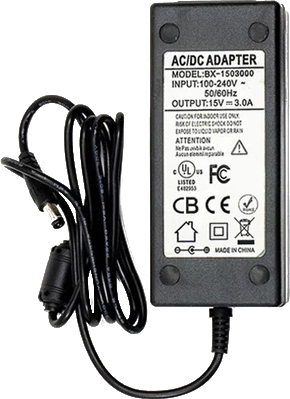
\includegraphics[width=\textwidth]{pictures/power-brick.png}
            \end{figure}
        \end{column}
    \end{columns}
\end{frame}

\begin{frame}{Découplage}
    \begin{itemize}
        \item $X_L \propto -X_C$
        \item Rajouter de la capacitance pour compenser l'inductance
        \item Plus ton fil est long, plus tu veux de capacitance
        \item Le power devrait provenir des condensateurs
        \item \textit{Couper le chemin d'inductance}
    \end{itemize}

    \pause
    \vfill
    \begin{center}
    \resizebox{0.8\textwidth}{0.5\textheight}{
    \ctikzset{bipoles/cuteinductor/height=0.15}
    \ctikzset{bipoles/cuteinductor/width=0.5}
    \begin{circuitikz}[american voltages]
        \draw [thick]
        (0, 0) to [short, *-] (10, 0)
        to [european resistor, l_=${LOAD}$] (10, 4)
        (0, 0) to [open, v<=$V$] (0, 4)
        to [short, *-] (1, 4)
        to [american inductor, l=$wire$, color=red] (5, 4)
        to [short] (6, 4)
        to [cute inductor, l=$pcb$, color=UDSgreenFierte] (10, 4)
        ;

        \draw [thick] (5, 0) to [C, l=$bulk$, color=red] (5, 4);
        \draw [thick] (6, 0) to [C, l_=$decoupling$, color=UDSgreenFierte] (6, 4);

        \draw[->, thick, red]
        (1, 3.5) to [out=0, in=180] (3.5, 3.5)
        to [out=0, in=90] (4.5, 2.5);
        \draw[->, thick, UDSgreenFierte]
        (6.5, 2.5) to [out=90, in=180] (7.5, 3.5)
        to [out=0, in=180] (8.5, 3.5)
        to [out=0, in=90] (9.5, 2.5);
    \end{circuitikz}
    }
    \end{center}
\end{frame}

\begin{frame}{Filtrage avancé d'une entrée d'alimentation}
    \begin{itemize}
        \item[] \textcolor{UDSgreenFierte}{\faTachometer*} ~Découplage permet de fournir un chemin de faible impédance aux signaux haute-vitesse
        \item[] \textcolor{UDSgreenFierte}{\faBatteryThreeQuarters} ~Bulk permet d'emmagasiner des charges et que le power provienne des condensateurs et non du fil
        \bigskip
        \item<2-> \textbf{Contrôler la propagation du bruit}
        \begin{itemize}
            \item<2->[] \textcolor{UDSgreenFierte}{\faArrowRight} ~Limiter le bruit au board
            \item<2->[] \textcolor{UDSgreenFierte}{\faArrowLeft} ~Limiter le bruit hors du board
            \item<2->[] \textcolor{UDSgreenFierte}{\faFileContract} ~Passer EMC
        \end{itemize}
        \item<3->[] \textcolor{UDSgreenFierte}{\faProjectDiagram} ~Principalement lorsque premier régulateur est un switching.
    \end{itemize}
\end{frame}

\begin{frame}{Rajouter des inductances}
    \begin{itemize}
        \item Rajouter de l'inductance permet de bien contrôler où va le bruit haute-fréquence.
        \item $X_L = 2\pi fL$
        \item Si $X_L > X_C$, le bruit va passer par $X_C$.
        \bigskip
        \item On vient de passer tout ce temps pour compenser l'inductance du fil d'alimentation
        \item<2-> Maintenant, on contrôle l'inductance!
        \begin{itemize}
            \item<2-> Les condensateurs de découplage fournissent la puissance haute fréquence
            \item<2-> Les condensateurs de bulk fournissent la puissance basse fréquence
            \item<2-> Les condensateurs de bulk rechargent les condensateurs de découplage
            \item<2-> L'alimentation fournit du power DC pour recharger les condensateurs de bulk
            \item<3->[] \hspace{-18pt} \textcolor{red}{\faBan}
                ~La bobine fait du bruit électromagnétique
        \end{itemize}
    \end{itemize}
\end{frame}

\begin{frame}{Filtre de 2e ordre contrôlé}
    \begin{columns}
        \begin{column}{0.5\textwidth}
            \centering
            $f = \dfrac{1}{2 \pi \sqrt{LC}}$
        \end{column}
        \begin{column}{0.5\textwidth}
            \centering
            $\zeta = \dfrac{1}{2 R_{_{LOAD}} \sqrt{LC}}$
        \end{column}
    \end{columns}

    \vfill

    \begin{center}
    \resizebox{0.8\textwidth}{!}{
    \ctikzset{bipoles/cuteinductor/height=0.15}
    \ctikzset{bipoles/cuteinductor/width=0.5}
    \begin{circuitikz}[american voltages]
        \draw [thick]
        (0, 0) to [short, *-] (12, 0)
        to [european resistor, l_=$R_{LOAD}$] (12, 4)
        (0, 0) to [open, v<=$V$] (0, 4)
        to [cute inductor, l=$wire$] (3, 4)
        to [american inductor, l=$L$, color=red] (5, 4)
        to [short] (9, 4)
        to [cute inductor, l=$pcb$] (12, 4)
        ;


        \draw [thick] (5.5, 0) to [C, l=$C$, color=red] (5.5, 4);
        \draw [thick] (8, 0) to [C, l=$bulk$] (8, 4);
        \draw [thick] (9, 0) to [C, l_=$decoupling$] (9, 4);

    \end{circuitikz}
    }
    \end{center}
\end{frame}

\begin{frame}{Damping factor}
    \centering
    $\zeta = \dfrac{1}{2 R_{_{LOAD}} \sqrt{LC}}$
    \vfill
    \begin{figure}
        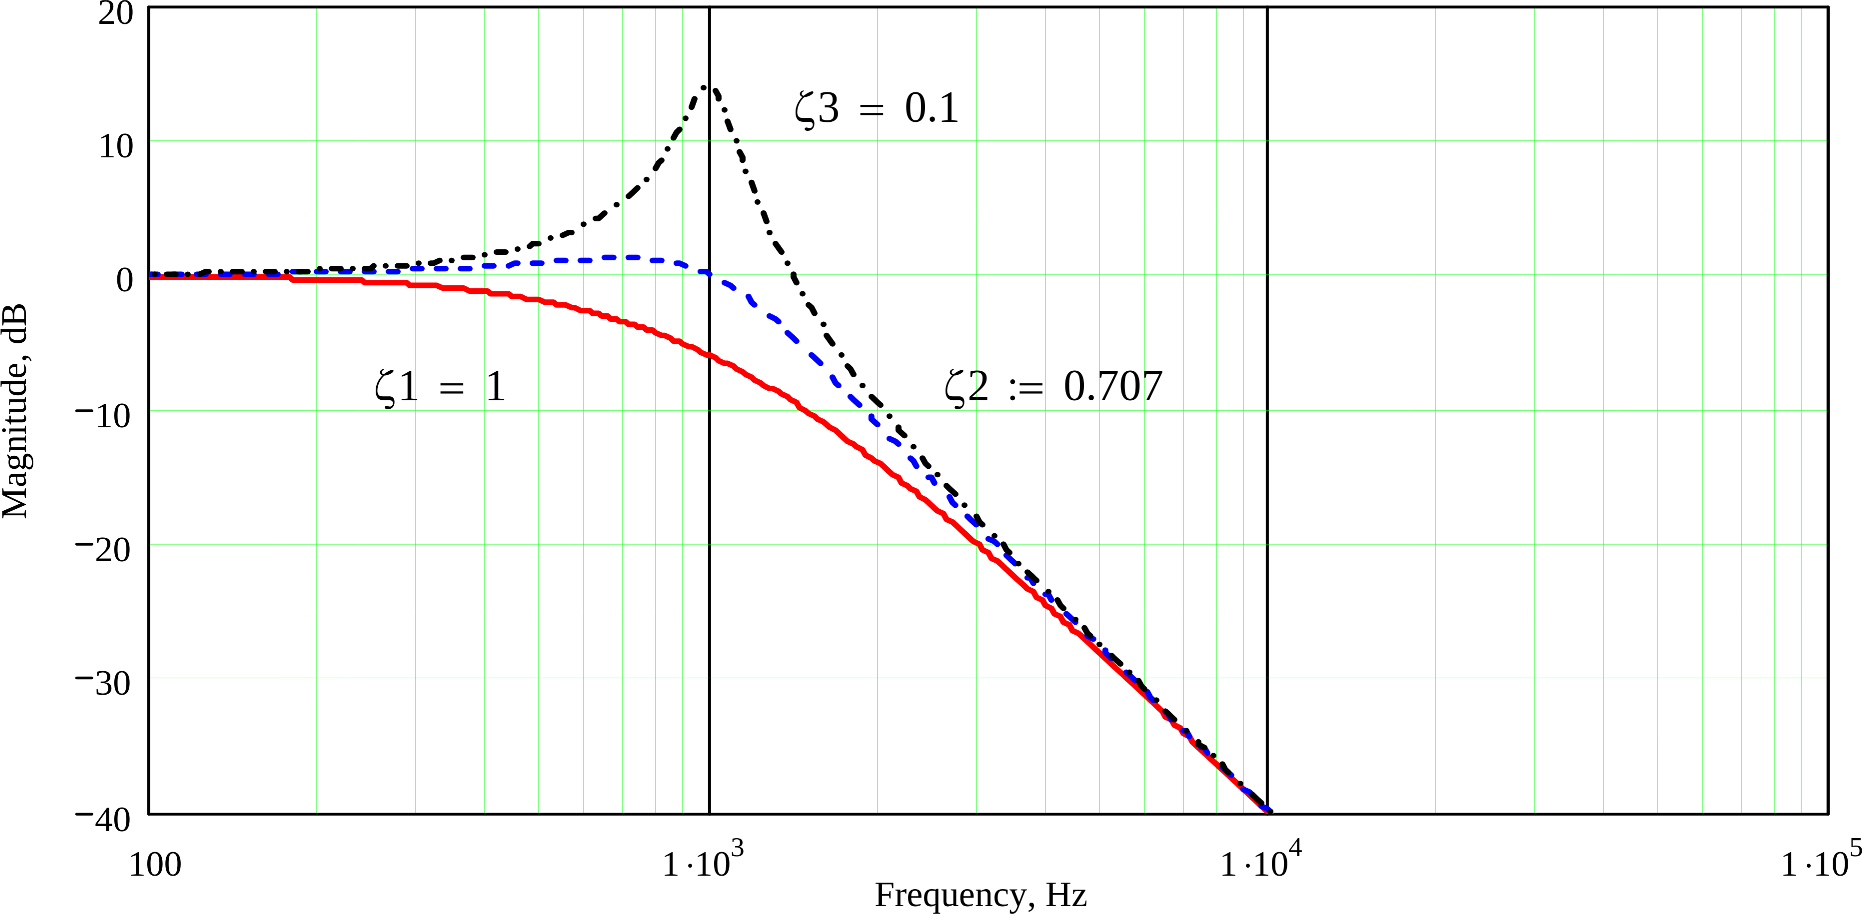
\includegraphics[width=\textwidth, height=0.7\textheight, keepaspectratio]{pictures/lc-filter-damping-factor.png}
    \end{figure}
\end{frame}

\begin{frame}{Common-Mode Noise}
    \begin{itemize}
        \item On veut contrôler les chemins de retour de courant
        \item \textbf{Le retour de courant est aussi important que l'aller}
    \end{itemize}
    \begin{center}
        \textcolor{UDSgreenFierte}{\faLongArrowAltRight}
        \textbf{Tous les grounds ne sont pas égaux!}
        \textcolor{UDSgreenFierte}{\faLongArrowAltLeft}
    \end{center}
    \pause
    \begin{itemize}
        \item \textit{Common-mode Noise}: Une partie du retour qui revient par ailleurs
        \item Donc pas autant de courant qui rentre que qui sort
    \end{itemize}
    \vfill
    \begin{figure}
        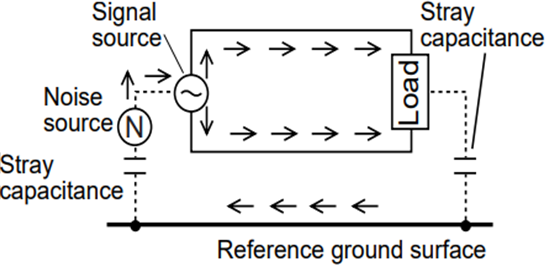
\includegraphics[width=0.75\textwidth, height=0.5\textheight, keepaspectratio]{pictures/common-mode-noise.png}
    \end{figure}
\end{frame}

\begin{frame}{Common-mode Choke}
    \begin{columns}
        \begin{column}{0.45\textwidth}
            \begin{itemize}
                \item[] \textcolor{UDSgreenFierte}{\faUnlink}
                    ~Essentiellement un transformateur
                \item[] \textcolor{UDSgreenFierte}{\faSync}
                    ~Permet d'égaler le flux qui passe à un point
                \item[] \textcolor{UDSgreenFierte}{\faExchange*}
                    ~Du courant est forcé par la bonne place si les courants ne sont pas égaux
                \bigskip
                \item[] \textcolor{UDSgreenFierte}{\faLongArrowAltRight}
                    ~Fournit un chemin de plus faible impédance vers là où on veut aller!
            \end{itemize}
        \end{column}
        \begin{column}{0.55\textwidth}
            \begin{figure}
                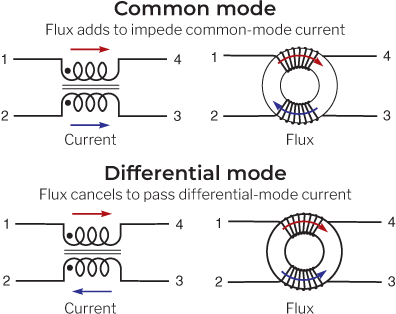
\includegraphics[width=\textwidth, height=0.75\textheight, keepaspectratio]{pictures/common-mode-choke.png}
            \end{figure}
        \end{column}
    \end{columns}
\end{frame}

\subsection{Filtrer un régulateur}

\begin{frame}{Pourquoi filtrer les régulateurs?}
    \begin{columns}
        \begin{column}{0.5\textwidth}
            \begin{itemize}
                \item Un régulateur linéaire n'a pas besoin d'être filtré
                \item Juste du bulk capacitance
                \bigskip
                \pause
                \item Un régulateur switching doit avoir du bulk \textit{et} du découplage
                \item Il faut éliminer le bruit à la fréquence de switching
                \item Mettre des condensateurs dont la \textit{fréquence de résonnance} est celle du switching.
            \end{itemize}
        \end{column}
        \begin{column}{0.5\textwidth}
            \begin{figure}
                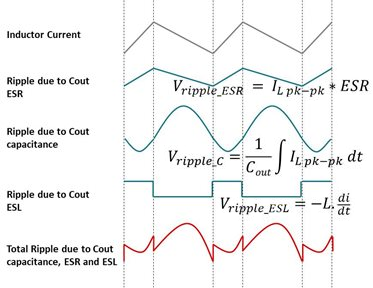
\includegraphics[width=\textwidth, height=0.75\textheight, keepaspectratio]{pictures/switching-psu-ripple-types.png}
            \end{figure}
        \end{column}
    \end{columns}
\end{frame}

\begin{frame}{Fréquence de résonnance d'un condensateur}
    \begin{itemize}
        \item Chaque condensateur a sa fréquence de résonnance
        \item Choisir le bon condensateur de découplage selon fréquence de résonnance du condensateur
        \item \textbf{Il faut offrir la plus faible impédance pour la fréquence visée}
    \end{itemize}
    \vspace{-12pt}
    \begin{columns}
        \begin{column}{0.5\textwidth}
            \begin{figure}
                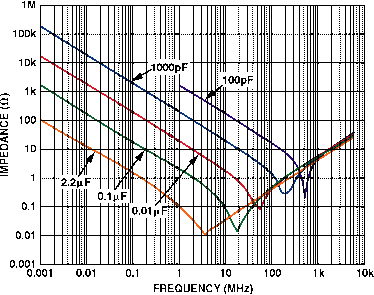
\includegraphics[width=\textwidth, height=0.55\textheight, keepaspectratio]{pictures/capacitor-resonant-frequency.png}
            \end{figure}
        \end{column}
        \begin{column}{0.5\textwidth}
            \begin{figure}
                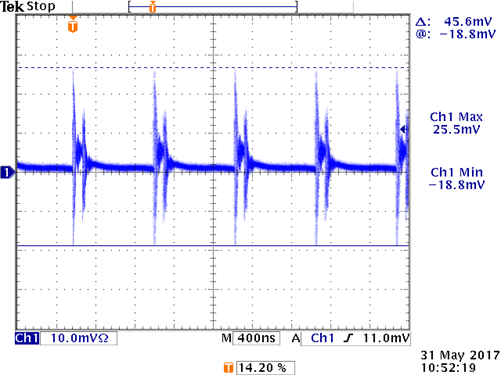
\includegraphics[width=0.95\textwidth, height=0.75\textheight, keepaspectratio]{pictures/switching-psu-ripple.png}
            \end{figure}
        \end{column}
    \end{columns}
\end{frame}


\subsection{Filtrer au IC}

\begin{frame}{Pourquoi filtrer au IC?}
    \vspace{-6pt}
    \begin{columns}
        \begin{column}{0.5\textwidth}
            \begin{center}
                \textbf{Protéger le IC du bruit}
            \end{center}
        \end{column}
        \begin{column}{0.5\textwidth}
            \begin{center}
                \textbf{Protéger les autres IC du bruit}
            \end{center}
        \end{column}
    \end{columns}
    \begin{columns}
        \begin{column}{0.5\textwidth}
            \begin{itemize}
                \item Un IC analogique est sensible au bruit
                \item Un IC digital est affecté aussi!
                \begin{itemize}
                    \item[] \textcolor{UDSgreenFierte}{\faNetworkWired} 
                        ~Communication
                    \item[] \textcolor{UDSgreenFierte}{\faWaveSquare} 
                        ~Clock
                    \item[] \textcolor{UDSgreenFierte}{\faBalanceScale} 
                        ~Stabilité
                \end{itemize}
            \end{itemize}
        \end{column}
        \begin{column}{0.5\textwidth}
            \vspace{-24pt}
            \begin{itemize}
                \item Un IC génère du bruit!
                \begin{itemize}
                    \item[] \textcolor{UDSgreenFierte}{\faNetworkWired} 
                        ~Communication
                    \item[] \textcolor{UDSgreenFierte}{\faWaveSquare} 
                        ~Clock
                    \item[] \textcolor{UDSgreenFierte}{\faRuler} 
                        ~Mesures
                \end{itemize}
            \end{itemize}
        \end{column}
    \end{columns}
    \vspace{-12pt}
    \begin{columns}
        \begin{column}{0.45\textwidth}
            \begin{figure}
                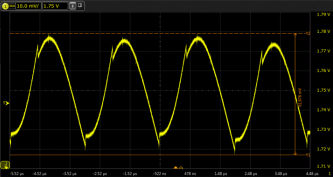
\includegraphics[width=0.9\textwidth, height=0.75\textheight, keepaspectratio]{pictures/oscilloscope-noise.png}
            \end{figure}
        \end{column}
        \begin{column}{0.45\textwidth}
            \begin{figure}
                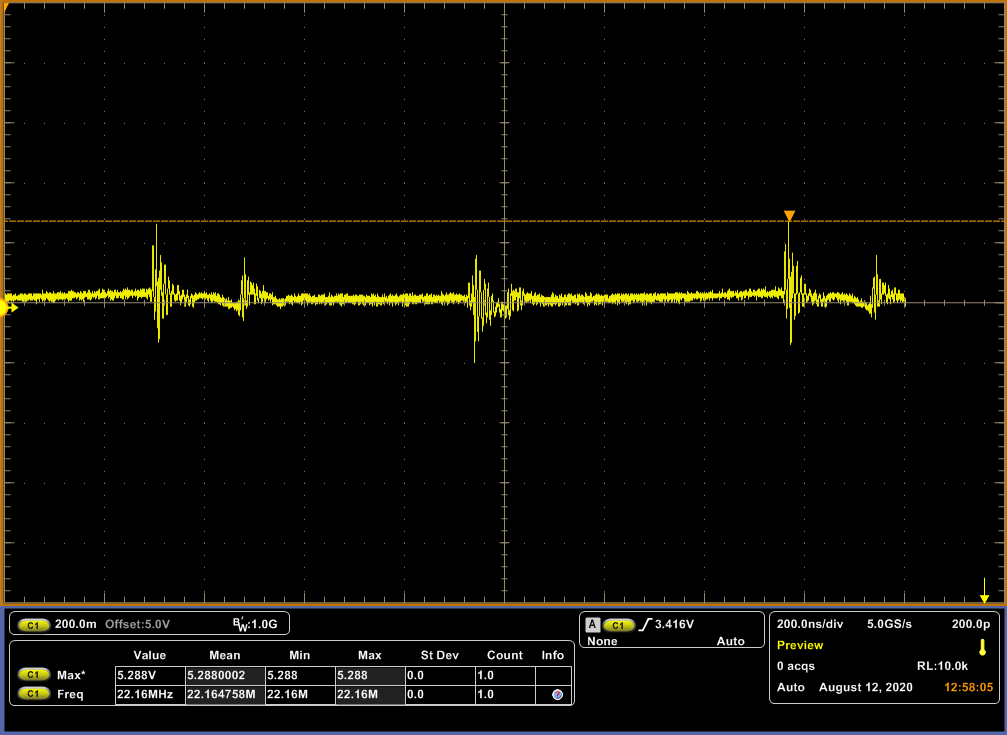
\includegraphics[width=\textwidth, height=0.55\textheight, keepaspectratio]{pictures/ic-noise.png}
            \end{figure}
        \end{column}
    \end{columns}
\end{frame}

\begin{frame}{Fréquences d'opération}
    \begin{columns}
        \begin{column}{0.5\textwidth}
            \begin{itemize}
                \item Chaque IC a plusieurs fréquences d'opération
                \begin{itemize}
                    \item[] \hspace{-20pt}\textcolor{UDSgreenFierte}{\faWaveSquare}
                        ~Fréquence des clocks
                    \item[] \hspace{-20pt}\textcolor{UDSgreenFierte}{\faNetworkWired}
                        ~Fréquences de communication
                    \item[] \hspace{-20pt}\textcolor{UDSgreenFierte}{\faRuler}
                        ~Fréquence d'acquisition de données
                \end{itemize}
            \end{itemize}
        \end{column}
        \begin{column}{0.55\textwidth}
            \begin{itemize}
                \item Chaque fréquence d'opération fait du bruit sur le power!
                \item \textbf{Il faut offrir le chemin de plus faible impédance au GND pour ces signaux haute-fréquence}
            \end{itemize}
        \end{column}
    \end{columns}
    \vspace{12pt}
    \pause
    \begin{itemize}
        \item Matcher la fréquence de résonnance avec la fréquence d'opération
    \end{itemize}

    \begin{figure}
        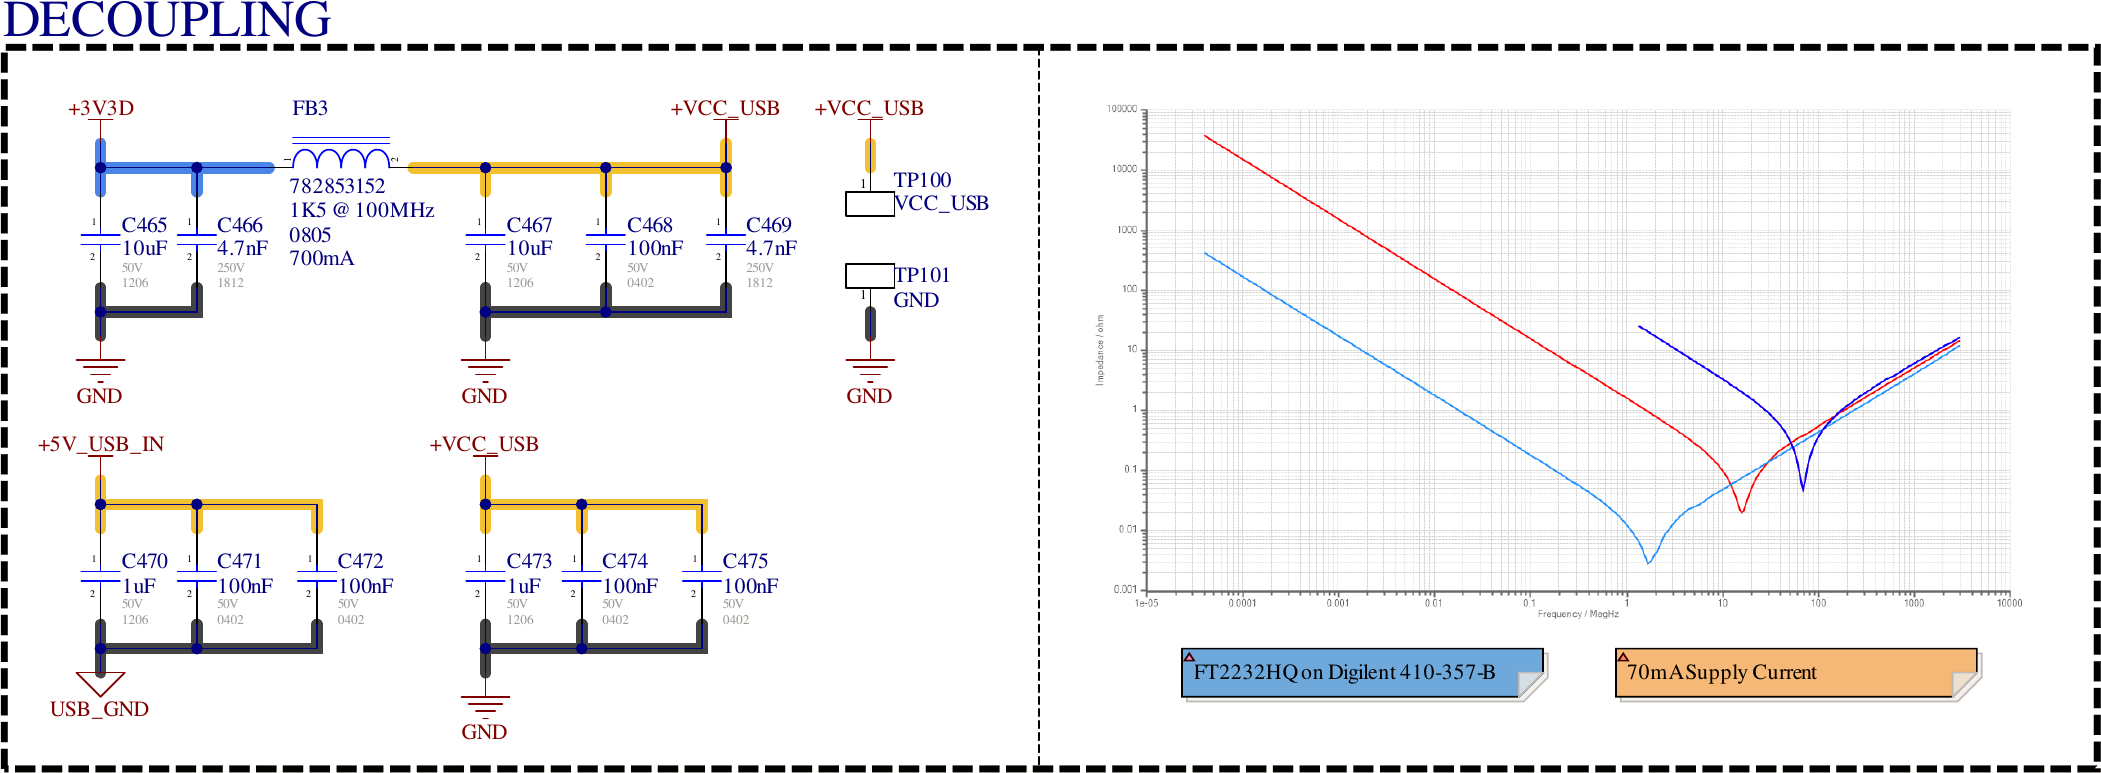
\includegraphics[width=0.8\textwidth, height=0.4\textheight, keepaspectratio]{pictures/decoupling-example-usb.png}
    \end{figure}
\end{frame}

\begin{frame}{Fréquence d'opération - Découplage}
    \begin{itemize}
        \item Chaque condensateur a une fréquence de résonnance où son impédance est la plus faible
        \item On veut offrir l'impédance la plus faible pour les fréquences d'opération
        \item Il faut donc un condensateur spécifique par fréquence d'opération
        \bigskip
        \item Le conseil habituel de $\SI{100}{\nano\farad}$ fonctionne parce que ça tourne autours des fréquences habituelles, mais c'est overall un mauvais conseil!
    \end{itemize}

    \begin{figure}
        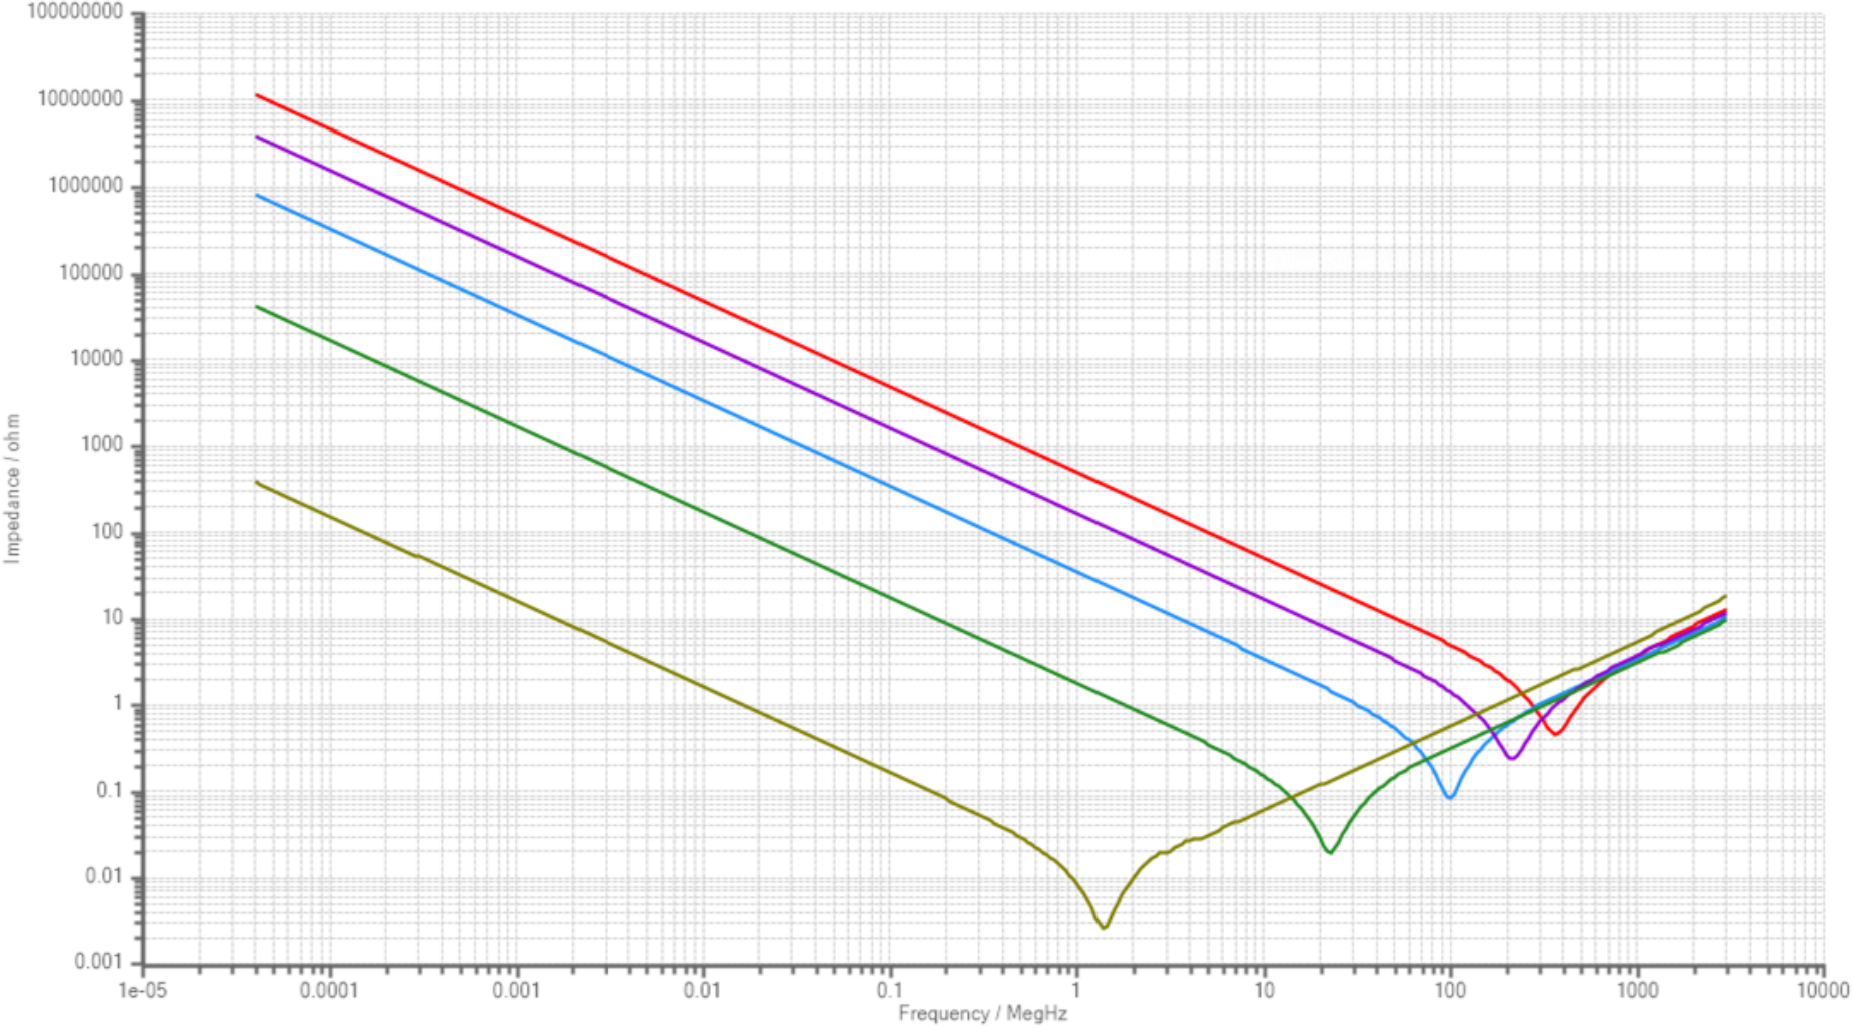
\includegraphics[width=0.6\textwidth, height=0.45\textheight, keepaspectratio]{pictures/decoupling-example-osc.png}
    \end{figure}
\end{frame}

\begin{frame}{Fréquence d'opération - Harmoniques}
    \begin{columns}
        \begin{column}{0.45\textwidth}
            \begin{itemize}
                \item Un onde carrée n'opère pas qu'à une seule fréquence
                \item Décomposer une onde dans toutes ses harmoniques
                \item Les harmoniques font partie du signal
                \bigskip
                \item Il faut rajouter des condensateurs pour les premières harmoniques!
            \end{itemize}
        \end{column}
        \begin{column}{0.55\textwidth}
            \begin{figure}
                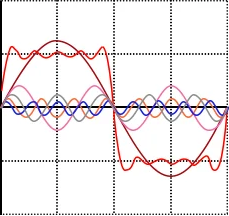
\includegraphics[width=\textwidth, height=0.75\textheight, keepaspectratio]{pictures/square-wave-harmonic-series.png}
            \end{figure}
        \end{column}
    \end{columns}
\end{frame}

\begin{frame}{Harmoniques supérieures}
    \begin{itemize}
        \item Les fréquences les plus élevées ($> \SI{1}{\giga\hertz}$) sont couvertes
        \item Le PCB lui-même agit comme un condensateur
        \item Il faut un power plane et un ground plane adjacents!
    \end{itemize}
    \begin{figure}
        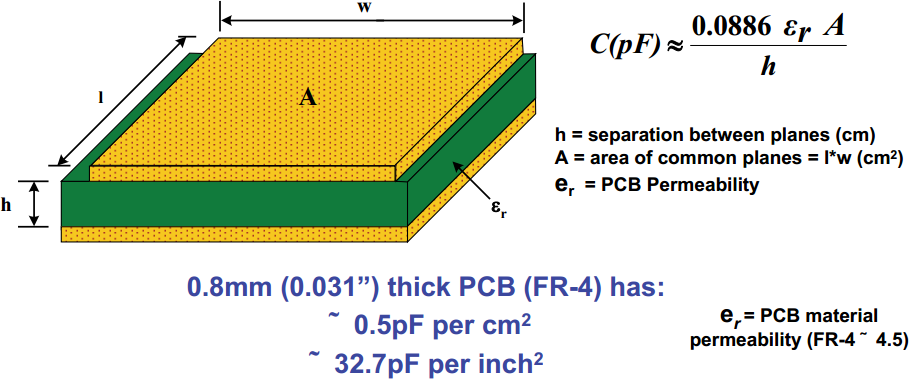
\includegraphics[width=\textwidth, height=0.55\textheight, keepaspectratio]{pictures/pcb-plane-capacitance.png}
    \end{figure}
\end{frame}

\begin{frame}{Découplage - Exemple}
    \begin{figure}
        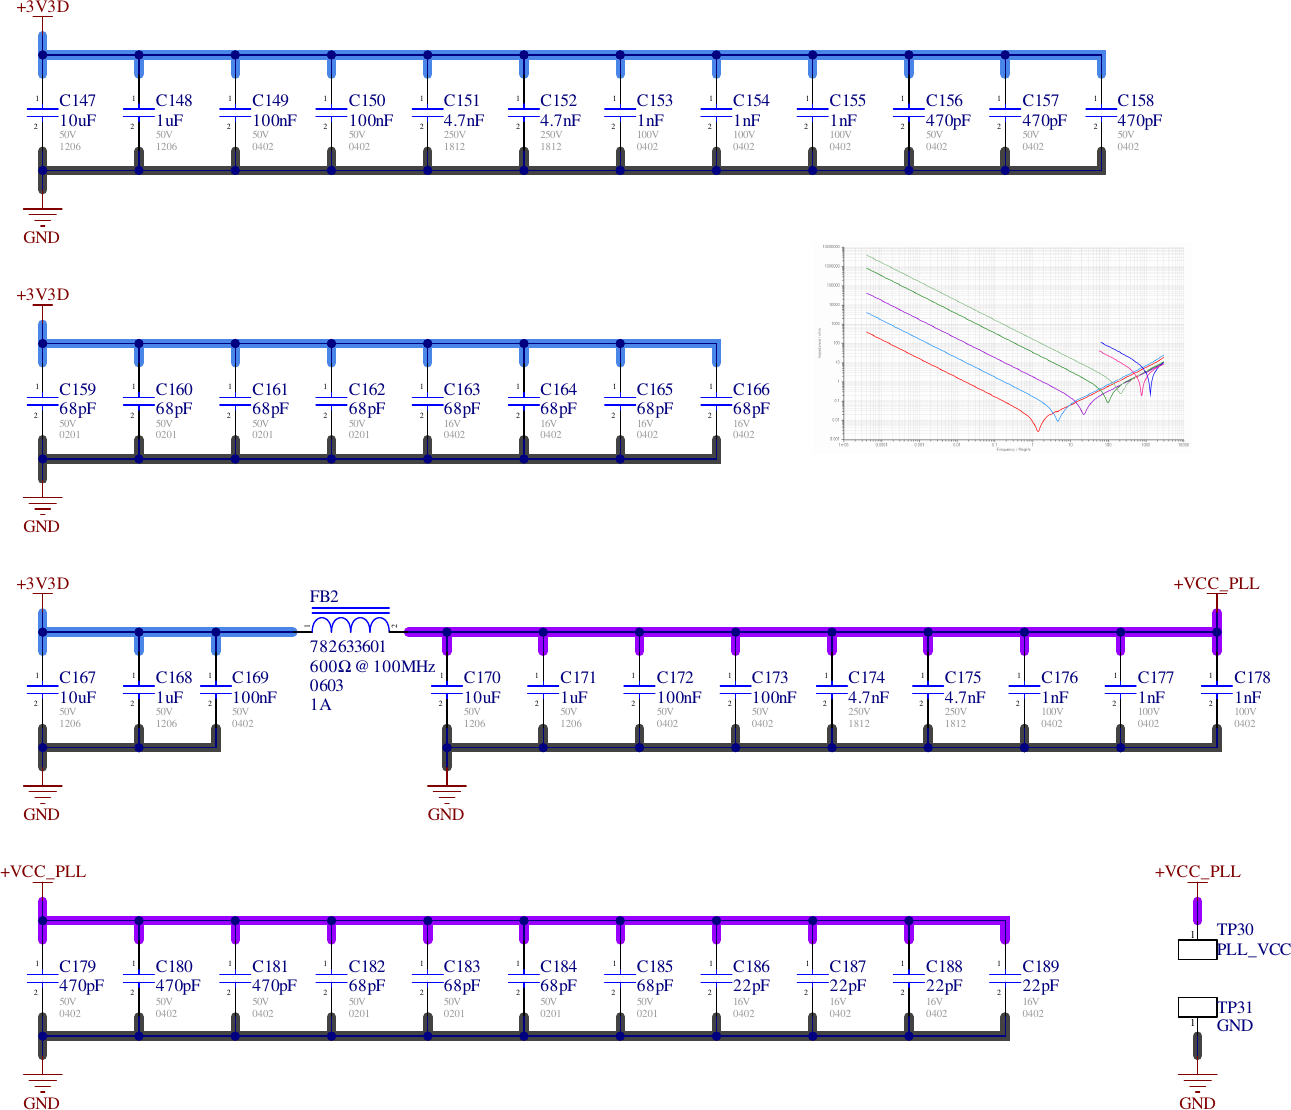
\includegraphics[width=\textwidth, height=0.75\textheight, keepaspectratio]{pictures/decoupling-example-pll.png}
    \end{figure}
\end{frame}

\begin{frame}{Où placer le découplage?}
    \begin{itemize}
        \item Le plus proche possible des pins d'alimentation du IC
        \item Le condensateur pour la fréquence la plus élevée le plus proche
        \item Briser le chemin d'inductance
        \item On ne veut pas que les hautes fréquences se propagent
        \item Faire des polygones - Chaque condensateur a un via
        \item \textbf{Offrir la plus faible impédance vers le GND pour les hautes fréquences}
    \end{itemize}
    \vspace{-12pt}
    \begin{columns}
        \begin{column}{0.7\textwidth}
            \begin{center}
            \resizebox{0.8\textwidth}{!}{
            \ctikzset{bipoles/cuteinductor/height=0.15}
            \ctikzset{bipoles/cuteinductor/width=0.5}
            \begin{circuitikz}[american voltages]
                \draw [thick]
                (0, 0) to [short, *-] (10, 0)
                to [european resistor, l_=${LOAD}$] (10, 4)
                (0, 0) to [open, v<=$V$] (0, 4)
                to [short, *-] (1, 4)
                to [american inductor, l=$pcb$, color=red] (5, 4)
                to [short] (6, 4)
                to [cute inductor, l=$tout\ petit$, color=UDSgreenFierte] (10, 4)
                ;

                \draw [thick] (5, 0) to [C, color=red] (5, 4);
                \draw [thick] (6, 0) to [C, color=UDSgreenFierte] (6, 4);

                \draw[->, thick, red]
                (1, 3.5) to [out=0, in=180] (3.5, 3.5)
                to [out=0, in=90] (4.5, 2.5);
                \draw[->, thick, UDSgreenFierte]
                (6.5, 2.5) to [out=90, in=180] (7.5, 3.5)
                to [out=0, in=180] (8.5, 3.5)
                to [out=0, in=90] (9.5, 2.5);
            \end{circuitikz}
            }
            \end{center}
        \end{column}

        \begin{column}{0.3\textwidth}
                \begin{figure}
                    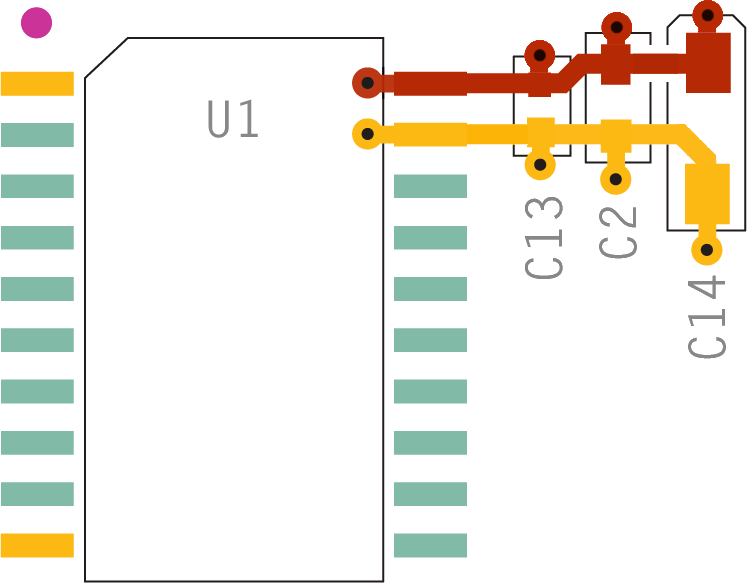
\includegraphics[width=\textwidth, height=0.66\textheight, keepaspectratio]{pictures/decoupling-placement.png}
                \end{figure}
        \end{column}
    \end{columns}
\end{frame}

\begin{frame}{Ferrite Beads}
    \begin{columns}
        \begin{column}{0.5\textwidth}
            \begin{itemize}
                \item \textbf{Ferrite Bead}
                \item Propriétés inductives
                \item Laisse passer le DC, bloque les hautes fréquences
                \bigskip
                \item Contrôler le chemin des signaux haute-fréquence
                \item Forcer à passer par les condensateurs
            \end{itemize}
        \end{column}

        \begin{column}{0.5\textwidth}
            \begin{center}
                \resizebox{0.4\textwidth}{!}{
                \begin{circuitikz}[]
                    \draw[thick] (0, 0) to[american inductor, name=L] ++(2,0);
                    \draw[thick, double] (L.core west) -- (L.core east);
                \end{circuitikz}
                }

                \begin{figure}
                    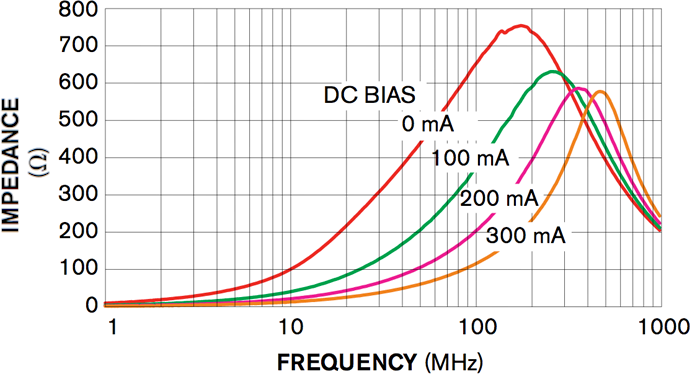
\includegraphics[width=\textwidth, height=0.66\textheight, keepaspectratio]{pictures/ferrite-bead-impedance.png}
                \end{figure}
            \end{center}
        \end{column}
    \end{columns}

    \begin{figure}
        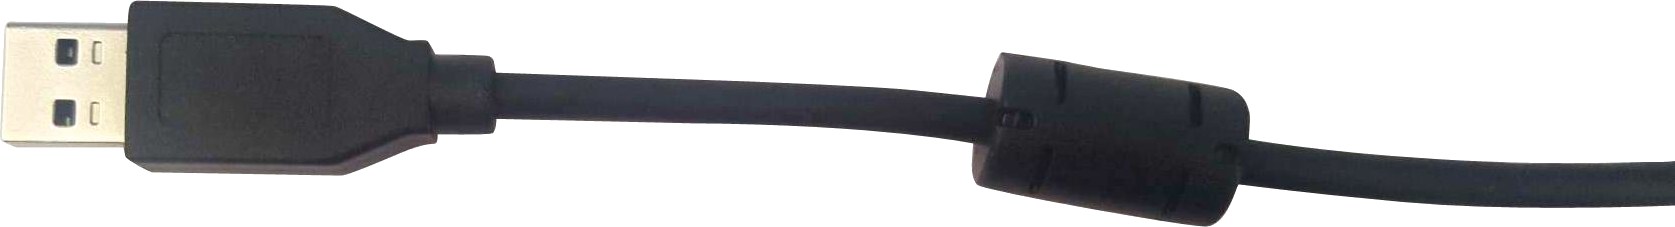
\includegraphics[width=\textwidth, height=0.75\textheight, keepaspectratio]{pictures/ferrite-bead-cable.png}
    \end{figure}
\end{frame}


\begin{frame}{Ferrite Bead - Fonctionnement}
    \begin{columns}
        \begin{column}{0.6\textwidth}
            \begin{itemize}
                \item Agit comme une résistance sur sa plage d'opération
                \item Utilisé comme une inductance dans un circuit
                \item Diffère dans sa courbe d'impédance caractéristique
            \end{itemize}
        \end{column}

        \begin{column}{0.4\textwidth}
            \begin{figure}
                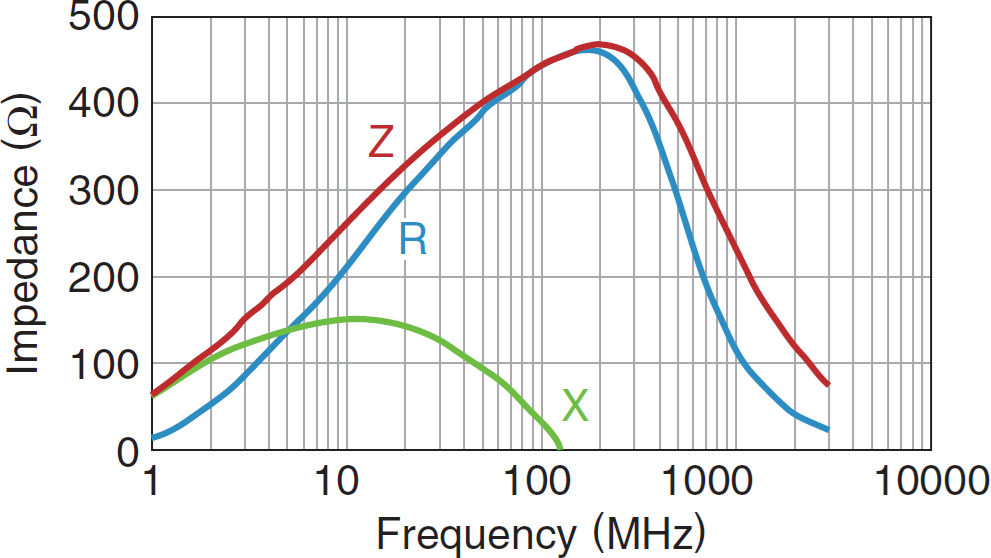
\includegraphics[width=\textwidth, height=0.75\textheight, keepaspectratio]{pictures/ferrite-bead-impedance-curve.png}
            \end{figure}
        \end{column}
    \end{columns}


    \pause
    \vspace{-48pt}
    \begin{columns}
    \begin{column}{0.7\textwidth}
        \begin{center}
        \resizebox{\textwidth}{!}{
        \ctikzset{bipoles/cuteinductor/height=0.15}
        \ctikzset{bipoles/cuteinductor/width=0.5}
        \begin{circuitikz}[american voltages]
            \draw [thick]
            (0, 0) to [short, *-] (10, 0)
            to [european resistor, l_=${LOAD}$] (10, 4)
            (0, 0) to [open, v<=$V$] (0, 4)
            to [short, *-] (1, 4)
            to [cute inductor, l=$pcb$] (3, 4)
            to [short] (4, 4)
            to [american inductor, l=$L$, name=L, color=red] (6.5, 4)
            to [short] (10, 4)
            ;

            \draw[thick, double, color=red] (L.core west) -- (L.core east);

            \draw [thick] (7, 0) to [C] (7, 4);
            \draw         (8, 0) to [C] (8, 4);
        \end{circuitikz}
        }
        \end{center}
    \end{column}
    \begin{column}{0.3\textwidth}
    \end{column}
    \end{columns}
\end{frame}


\begin{frame}{Pi Filter}
    \begin{itemize}
        \item Ajouter les mêmes condensateurs de chaque côté de la ferrite
        \item Plus de filtration
    \end{itemize}
    \vfill
    \begin{center}
    \resizebox{0.8\textwidth}{!}{
    \ctikzset{bipoles/cuteinductor/height=0.15}
    \ctikzset{bipoles/cuteinductor/width=0.5}
    \begin{circuitikz}[american voltages]
        \draw [thick]
        (0, 0) to [short, *-] (10, 0)
        to [european resistor, l_=${LOAD}$] (10, 4)
        (0, 0) to [open, v<=$V$] (0, 4)
        to [short, *-] (1, 4)
        to [cute inductor, l=$pcb$] (3, 4)
        to [short] (5, 4)
        to [american inductor, l=$L$, name=L] (7, 4)
        to [short] (10, 4)
        ;

        \draw[thick, double] (L.core west) -- (L.core east);

        \draw [thick] (4, 0) to [C, color=red] (4, 4);
        \draw         (5, 0) to [C, color=red] (5, 4);
        \draw [thick] (7, 0) to [C] (7, 4);
        \draw         (8, 0) to [C] (8, 4);
    \end{circuitikz}
    }
    \end{center}
\end{frame}

\begin{frame}{Ferrite Bead - Désavantages}
    \begin{columns}
        \begin{column}{0.5\textwidth}
            \textbf{Limite de courant}
            \begin{itemize}
                \item Résistance $\neq \SI{0}{\ohm}$
                \begin{itemize}
                    \item DC bias
                    \item Chauffe
                \end{itemize}
                \item Saturation de l'inductance
            \end{itemize}
        \end{column}
        \pause
        \begin{column}{0.5\textwidth}
            \textbf{Impédance}
            \begin{itemize}
                \item Affecte les courbes d'impédance
                \item Peut introduire du ringing
                \begin{itemize}
                    \item<3-> $\zeta = \dfrac{1}{2 \color{red}{R_{_{LOAD}}} \color{black}{\sqrt{LC}}}$
                \end{itemize}
            \end{itemize}
        \end{column}
    \end{columns}

    \vfill
    \begin{figure}
        \includegraphics<3->[width=\textwidth, height=0.55\textheight, keepaspectratio]{pictures/ferrite-bead-ringing.png}
    \end{figure}
\end{frame}

\begin{frame}{Ferrite Bead - Damping}
    \begin{figure}
        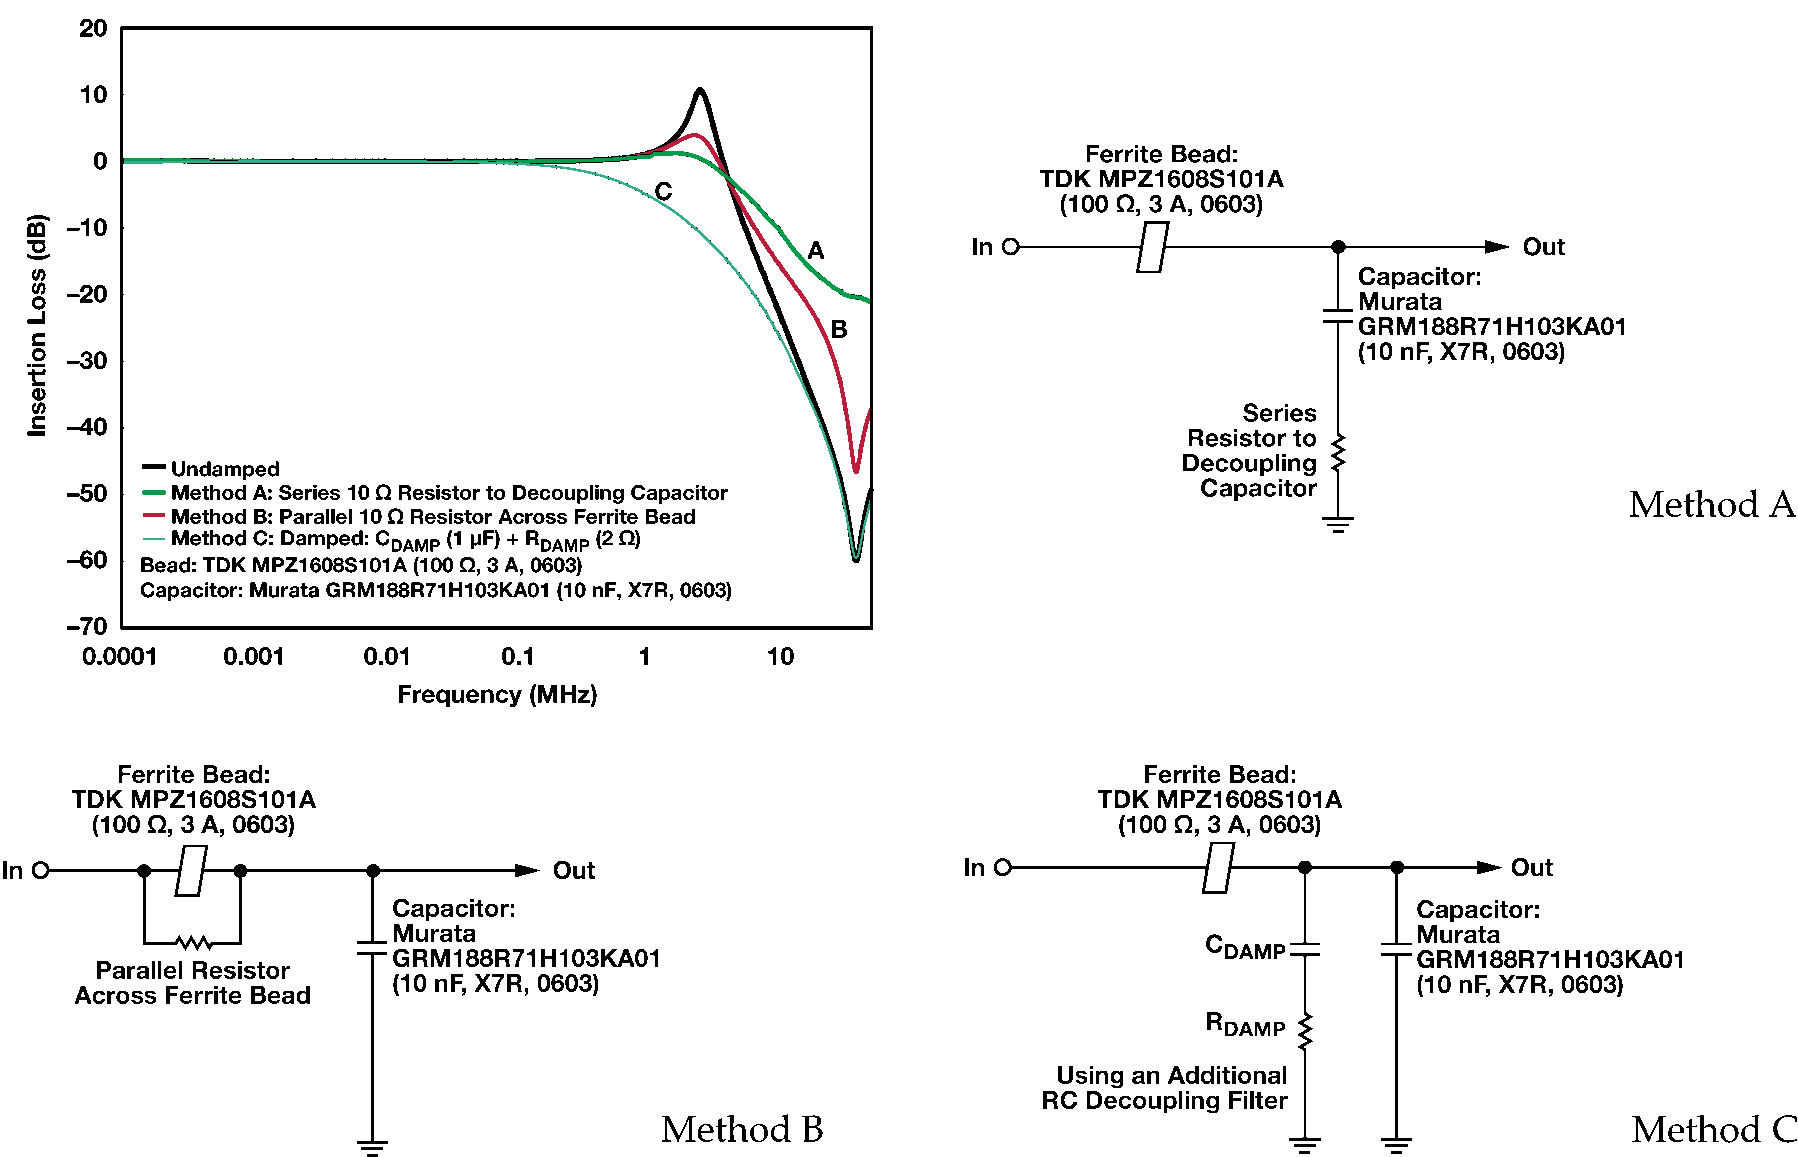
\includegraphics[width=\textwidth, height=0.75\textheight, keepaspectratio]{pictures/ferrite-bead-ringing-damping.png}
    \end{figure}
    \href{https://www.analog.com/en/resources/analog-dialogue/articles/ferrite-beads-demystified.html}{Analog Devices - Ferrite Beads Demystified}
\end{frame}

\begin{frame}{Plusieurs pins de power}
    \begin{itemize}
        \item Souvent plusieurs pins de power par IC
        \item Chaque pin a besoin de tous les condensateurs pour supporter toutes les fréquences
        \item Exception: Gros condensateurs ($\geq \SI{1}{\micro\farad}$)
        \item Besoin d'une seule ferrite bead
    \end{itemize}
    \begin{figure}
        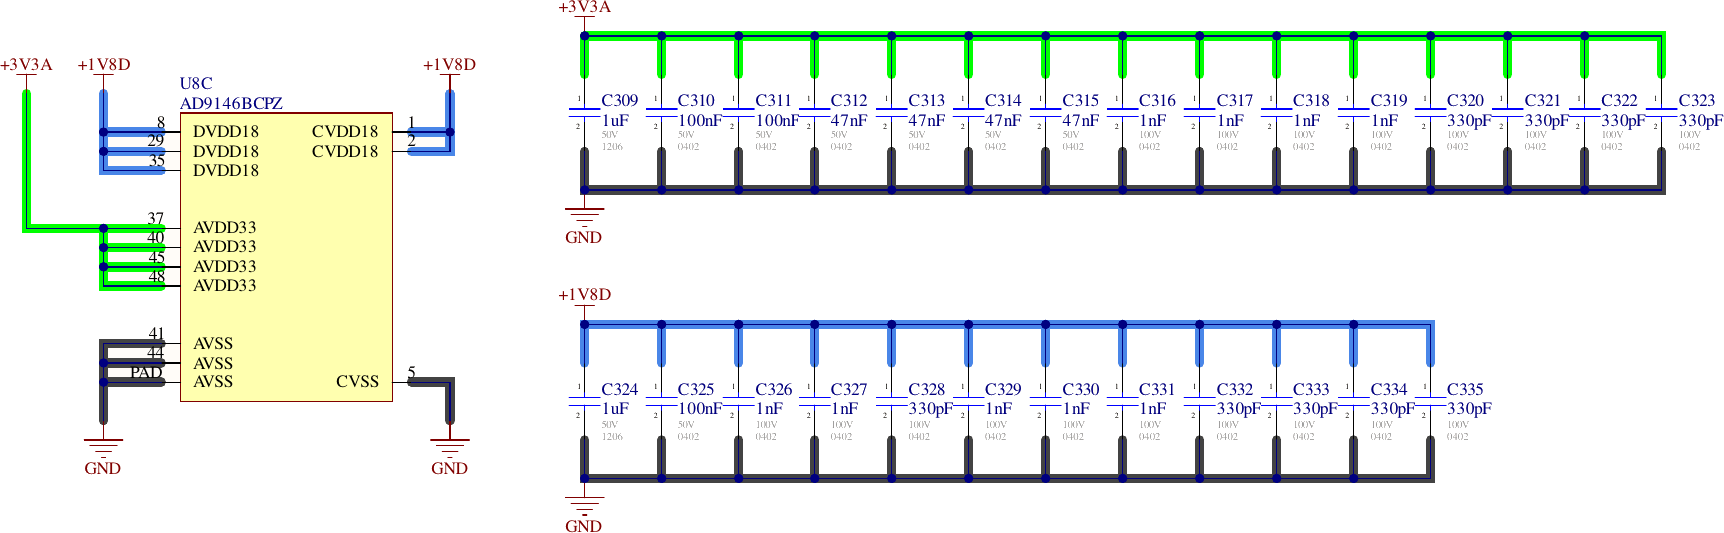
\includegraphics[width=\textwidth, height=0.75\textheight, keepaspectratio]{pictures/decoupling-example-dac.png}
    \end{figure}
\end{frame}


\subsubsection{Filtration Complète}

\begin{frame}{Filtration complète - Circuit électrique}
    \begin{center}
        \resizebox{0.8\textwidth}{!}{
        \begin{tikzpicture}[
            block/.style = {rectangle, draw, minimum height=1cm,        minimum width=2.5cm, align=center},
            node distance=0.8cm and 0.6cm,
            >={Stealth[round]}
        ]
        
        % Nodes
        \node[coordinate] (inlabel) {};

        \only<1-2> {
            \node[block, right=of inlabel] (prot) {Protections};
            \node[block, right=of prot] (choke) {Chokes};
            \node[block, right=of choke] (cap) {Bulk\\Capacitance};

            \node[block, below=of prot] (sw) {Switching Regulator\\+ Decoupling};
            \node[block, right=of sw] (pi) {Pi Filter};
            \node[block, right=of pi] (ic) {Integrated\\Circuit};
        }
        \only<3> {
            \node[block, right=of inlabel, color=gray]
                (prot) {Protections};
            \node[block, right=of prot, color=green]
                (choke) {Chokes};
            \node[block, right=of choke, color=magenta]
                (cap) {Bulk\\Capacitance};

            \node[block, below=of prot, color=red]
                (sw) {Switching Regulator\\+ Decoupling};
            \node[block, right=of sw, color=cyan]
                (pi) {Pi Filter};
            \node[block, right=of pi, color=blue]
                (ic) {Integrated\\Circuit};
        }

        \node[coordinate, right=of ic] (outlabel) {};

        % Input arrow with label
        \draw[->] ($(inlabel)+(-0.75,0.0)$) -- (prot.west) node[midway, above] {Input};

        % Top row
        \draw[->] (prot) -- (choke);
        \draw[->] (choke) -- (cap);

        % Segmented down to second row
        \draw[->] 
        (cap.east)      
        -- ++(0.5, 0)     
        -- ++(0, -0.85)    
        -| (sw.north);


        % Bottom row
        \draw[->] (sw) -- (pi);
        \draw[->] (pi) -- (ic);

        % Output arrow with label
        \draw[->] (ic.east) -- ++(1.25,0) node[midway, above] {Load};


        \only<1> {
            \node[above=1 of prot, draw, inner sep=5pt, scale=0.5] (zoom) {
                \begin{tikzpicture}
                    % Nodes
\node[coordinate] (inlabel) {};
\node[block, right=of inlabel] (scp) {Short-circuit\\       Protection};
\node[block, right=of scp] (tvs) {Transient Voltage\\       Suppression};
\node[block, right=of tvs] (rvp) {Reverse Voltage\\     Protection};

\node[block, below=of scp] (uvlo) {Undervoltage\\Lockout};
\node[block, right=of uvlo] (ss) {Soft Start};
\node[block, right=of ss] (cm) {Current\\Measurement};
\node[coordinate, right=of cm] (outlabel) {};

% Input arrow with label
\draw[->] ($(inlabel)+(-0.75,0.0)$) -- (scp.west) node[     midway, above] {Input};

% Top row
\draw[->] (scp) -- (tvs);
\draw[->] (tvs) -- (rvp);

% Segmented down to second row
\draw[->] 
(rvp.east)      
-- ++(0.5, 0)     
-- ++(0, -0.85)    
-| (uvlo.north);


% Bottom row
\draw[->] (uvlo) -- (ss);
\draw[->] (ss) -- (cm);

% Output arrow with label
\draw[->] (cm.east) -- ++(1.25,0) node[midway, above] {Load};
                \end{tikzpicture}
            };

            \draw (prot.north west) -- (zoom.south west);
            \draw (prot.north east) -- (zoom.south east);
        }
        \end{tikzpicture}
        }


    \vfill
    \pause

    \hspace{-14pt}
    \resizebox{1.025\textwidth}{!}{
    \ctikzset{bipoles/cuteinductor/height=0.15}
    \ctikzset{bipoles/cuteinductor/width=0.5}
    \ctikzset{bipoles/resistor/height=0.15}
    \ctikzset{bipoles/resistor/width=0.5}
    \begin{circuitikz}[
            american voltages,
            american inductors,
            block/.style = {rectangle, draw, minimum height=1cm,        minimum width=2.5cm, align=center},
            node distance=0.8cm and 0.6cm,
            >={Stealth[round]}
        ]]
        \only<2> {
            \node[block] (prot) at (4, 5) {Protections};
        }
        \only<3> {
            \node[block, color=gray] (prot) at (4, 5) {Protections};
        }

        % Circuit setup and wire inductance
        \draw [thick]
        (0, 0) to [open, v<=$V$] (0, 5)
        to [short, *-] (0.5, 5)
        to [cute inductor, l=$wire$] (2.5, 5)
        to [short] (prot.west)
        ;

        % Common-mode Choke
        \draw [thick]
        (7.5, 2.5) node[transformer core, rotate=90, transform shape](choke)
            {
                \begin{minipage}{4cm}
                    \centering
                    \rotatebox{-90}{
                        \large{Choke}
                    }
                    \rotatebox{-90}{
                        \hspace{-32pt}
                        \large{Common-Mode}
                    }
                \end{minipage}
            }
        (choke.A1) to [short] (choke.A1 |- 0, 0)
        to [short, -*] (0, 0)
        (choke.A2) to [short] (choke.A2 |- 0, 0)
        (choke.B1) to [short] (choke.B1 |- 0, 5)
        to [short] (prot.east)
        (choke.B2) to [short] (choke.B2 |- 0, 5)
        ;

        % Bulk Capacitance
        \draw[thick]
        (10, 5) to [curved capacitor, v=$ $, *-*] (10, 0)
        (11, 5) to [C, *-*] (11, 0);

        % Regulator
        \ctikzset{multipoles/dipchip/width=2}
        \draw (16.75, 5) node[dipchip,
            num pins=6,
            hide numbers,
            external pins width=0.3,
            external pad fraction=4,
            anchor=bpin 1,
            thick]
            (reg){L6982};
        \node [right, font=\tiny] at (reg.bpin 1) {VIN};
        \node [right, font=\tiny] at (reg.bpin 2) {EN};
        \node [right, font=\tiny] at (reg.bpin 3) {VCC};
        \node [left,  font=\tiny] at (reg.bpin 4) {GND};
        \node [left,  font=\tiny] at (reg.bpin 5) {FB};
        \node [left,  font=\tiny] at (reg.bpin 6) {SW};

        % Regulator Decoupling
        \draw[thick]
        (13, 5) to [C, *-*] (13, 0)
        (23.5, 5) to [C, *-*] (23.5, 0)
        ;

        % Regulator Circuit
        \draw[thick]
        (reg.pin 1) to [short] (choke.B2 |- 0, 5)
        (reg.pin 3) to [short] (reg.pin 3 -| 16, 0)
        to [C, -*] (16, 0)

        (reg.pin 2) to [short, -*] (reg.pin 2 -| 15, 0)
        to [R, -*] (15, 0)
        (reg.pin 2 -| 15, 0) to [R] (reg.pin 2 -| 13.5, 0)
        to [short, -*] (13.5, 5)

        (reg.pin 4) to [short] (reg.pin 4 -| 20.25, 0)
        to [short, -*] (20.25, 0)

        (reg.pin 5) to [short, -*] (reg.pin 5 -| 21, 0)
        to [R, -*] (21, 0)
        (reg.pin 5 -| 21, 0) to [R] (reg.pin 5 -| 23, 0)
        to [short, -*] (23, 5)

        (reg.pin 6) to [L, l=$L$] (23, 5)
        ;


        % Integrated Circuit
        \draw (34, 5) node[qfpchip,
            num pins=16,
            hide numbers,
            external pins width=0.3,
            external pad fraction=4,
            anchor=bpin 1,
            thick]
            (ic){STM32};
        \node [right, font=\tiny] at (ic.bpin 1)  {VDD};
        \node [right, font=\tiny] at (ic.bpin 4)  {GND};
        \node [left,  font=\tiny] at (ic.bpin 9)  {GND};
        \node [left,  font=\tiny] at (ic.bpin 12) {VDD};

        % IC Decoupling
        \draw[thick]
        (ic.pin 1) to [short] (ic.pin 1 -| 31, 5)
        (ic.pin 4) to [short] (ic.pin 4 -| 31, 0)
                   to [short, -*] (31, 0)
        (ic.pin 1 -| 33, 0) to [C, *-*] (ic.pin 4 -| 33, 0)
        (ic.pin 1 -| 32, 0) to [C, *-*] (ic.pin 4 -| 32, 0)
        (ic.pin 1 -| 31, 0) to [C, *-*] (ic.pin 4 -| 31, 0)
        ;
        \draw[thick]
        (ic.pin 12) to [short] (ic.pin 12 -| 40, 5)
        (ic.pin 9)  to [short] (ic.pin 9 -| 40, 0)
                    to [short] (40, 0)
                    to [short] (choke.A2 |- 0, 0)
        (ic.pin 12 -| 38, 0) to [C, *-*] (ic.pin 9 -| 38, 0)
        (ic.pin 12 -| 39, 0) to [C, *-*] (ic.pin 9 -| 39, 0)
        (ic.pin 12 -| 40, 0) to [C, -*]  (ic.pin 9 -| 40, 0)
        ;


        % Pi Filter
        \draw[thick]
        (23, 5) to [short] (28, 5)
                to [L, l=$FB$, name=fb] (30.5, 5)
                to [short] (ic.pin 1);
        \draw[thick, double] (fb.core west) -- (fb.core east);

        \draw[thick]
        (28, 5) to [C, *-*] (28, 0)
        (27, 5) to [C, *-*] (27, 0)
        (26, 5) to [C, *-*] (26, 0)
        ;

        \draw[thick]
        (30.5, 5) to [short, *-] (30.5, 6.5)
                  to [short]     (38.5, 6.5)
                  to [short, -*] (38.5, 5);

        % Boxes
        \only<3> {
            \draw[dashed, ultra thick, rounded corners, color=green] (3, 3.5) rectangle (9, 1.5);

            \draw[dashed, ultra thick, rounded corners, color=magenta] (9.25, 6) rectangle (11.75, -1);

            \draw[dashed, ultra thick, rounded corners, color=red] (12, 6) rectangle (24.5, -1);

            \draw[dashed, ultra thick, rounded corners, color=cyan] (24.75, 6) rectangle (33.5, 1);

            \draw[dashed, ultra thick, rounded corners, color=blue] (30, 7) rectangle (41, -1);

        }

    \end{circuitikz}
    }
    \end{center}
\end{frame}


\begin{frame}{Exemple - Régulateurs}
    \begin{figure}
        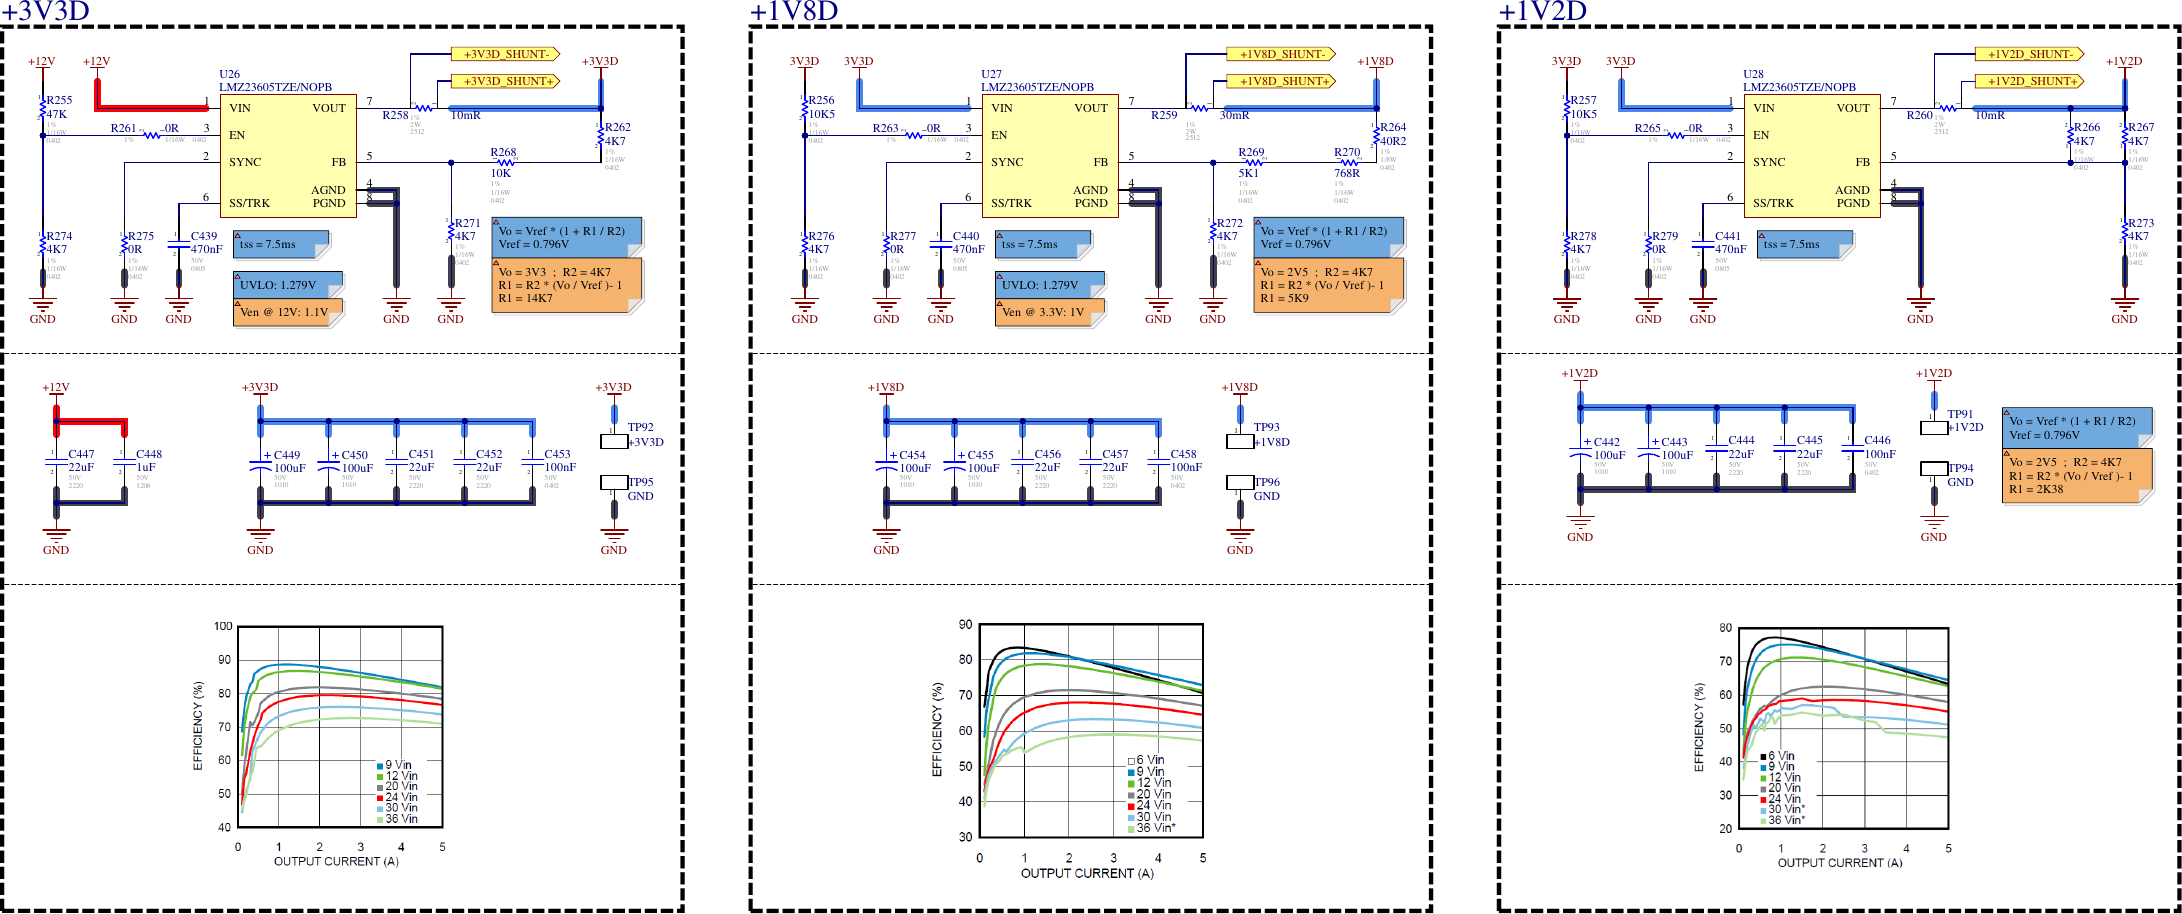
\includegraphics[width=\textwidth, height=0.75\textheight, keepaspectratio]{pictures/power-example-3v3.png}
    \end{figure}
\end{frame}


\begin{frame}{Exemple - Input \& Découplage}
    \begin{figure}
        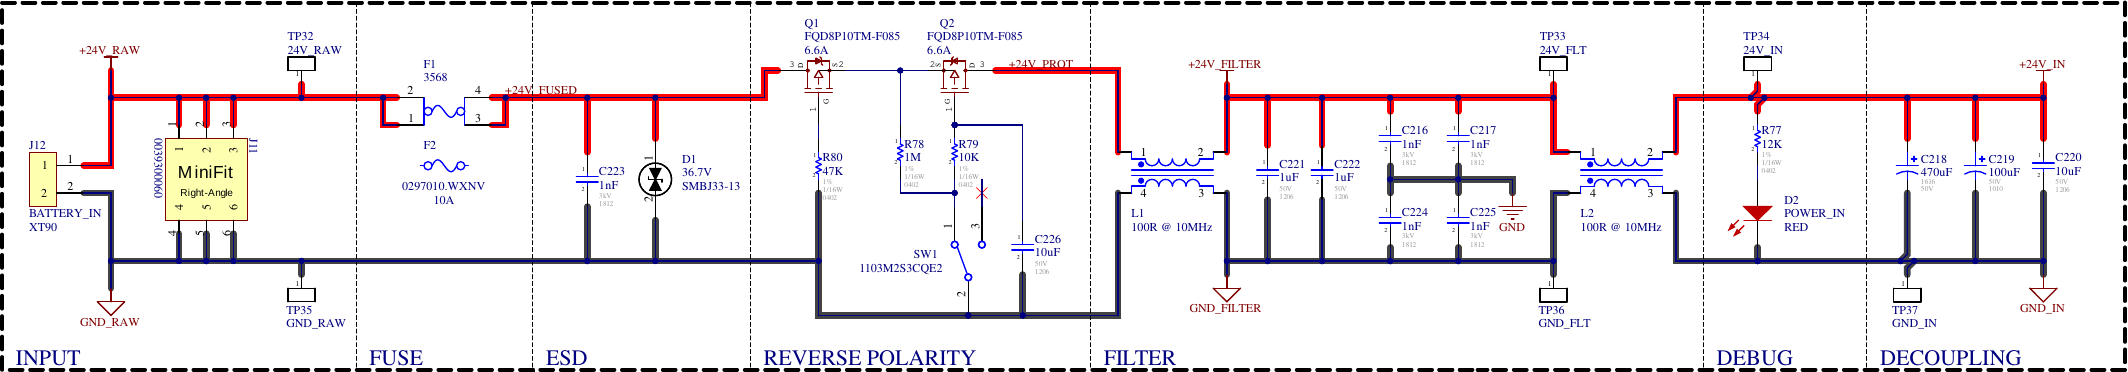
\includegraphics[width=\textwidth, height=0.75\textheight, keepaspectratio]{pictures/power-example-input.png}
    \end{figure}

    \begin{figure}
        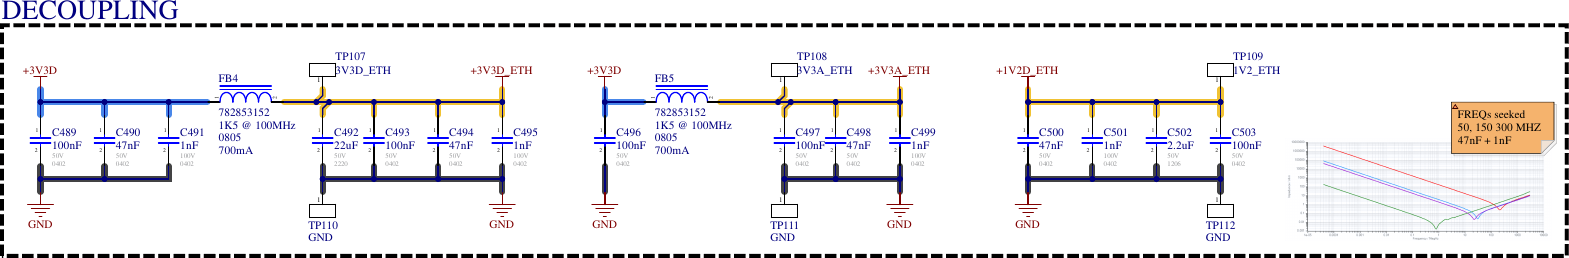
\includegraphics[width=\textwidth, height=0.75\textheight, keepaspectratio]{pictures/decoupling-example-eth.png}
    \end{figure}
\end{frame}